\documentclass{article}

%%%%%%%% SKYEPAPHORA %%%%%%%%
\usepackage[margin=1in]{geometry} 
\usepackage{amsmath,amsthm,amssymb,amsfonts}
\usepackage{xcolor}
\usepackage{cancel}
\usepackage[framemethod=tikz]{mdframed}
\usepackage{mathtools}
\usepackage{bm}
\usepackage{caption}
\usepackage{graphicx}
\usepackage{enumerate}
\usepackage{setspace}
\usepackage{listings}
\usepackage{multicol}
\usepackage{textcomp}
\usepackage{centernot}
\usepackage{bbm}
\usepackage{mathrsfs}
\usepackage{hyperref}
\hypersetup{
    colorlinks=false,
    linkcolor=blue
    }

\setlength{\fboxsep}{5pt}
% \setlength{\parindent}{0pt}

\newcommand{\define}{\ensuremath \stackrel{\text{def}}{=}}
\newcommand{\Var}{\ensuremath \text{Var}}
\newcommand{\Cov}{\ensuremath \text{Cov}}
\newcommand{\E}{\ensuremath \text{E}}
\newcommand{\myrule}{\rule{\linewidth}{0.5pt}}

\definecolor{gold}{HTML}{A05000}
\definecolor{redd}{HTML}{C00000}
\definecolor{bluu}{HTML}{0000C0}
\definecolor{gren}{HTML}{00B000}

\definecolor{salt}{HTML}{FBFAF9}
\definecolor{pepper}{HTML}{251F18}

\begin{document}
\pagecolor{salt}\color{pepper}

% --- Curvy BCMTFSE ---------
\section{Further Modifications to the BCMTFSE}
One disadvantage of the BCMTFSE is that the extrapolation taking place at either time-endpoint of the MTFSE is \textit{linear.} This disregards what curvature (with respect to time) might be present in the true Time Frequency Spectrum within those time-boundary regions. Moreover, this extrapolation is entirely dependent on the time derivative of the MTFSE at those solitary endpoints. For any column of the MTFSE, a lack of smoothness adjacent to these endpoints may result in wildly steep or shallow extrapolations, perhaps of the wrong signature $-$ all due to a ``bump in the road," so to speak.

FIGURE

\section{Boundary Correction for the MTFSE using Second-Order Taylor Approximations}
One way to account for possible time-boundary curvature is to extend the estimate into these regions by way of \textit{second} order Taylor approximations. This approach is not without its disadvantages. In fact, by incorporating the MTFSE's second time derivative into the mix, we obtain an estimate \textit{less smooth} than the original BCMTFSE. An opportunity to apply non-linear extrapolations in this context is, nevertheless, worth investigating.

\subsection{Constructing the CBCMTFSE}
Recall that, according to Non-Stationary Quadratic Inverse Theory, the TFS of a non-stationary process may be approximated by (??), with accompanying eigenvalue equation (??). Recall, further, that this may be applied when the TFS is restricted to a block $b$.
\begin{flalign}
        S_b(t,f) &\approx \sum_{l=0}^{L_b} a_{l,b}(f)A_l(t-b) 
    \intertext{We now consider an approximation formed by the 1st \textit{3} terms of $S_b(t,f)$'s Taylor expansion (rather than the first \textit{2,} as per the technique from section (??)).}
        S_b(t,f) \approx  S_b(t_b,f) 
                &+ S^{(1)}(t_b,f)(t-t_b) + \frac{1}{2}S^{(2)}(t_b,f)^2
\end{flalign}
Similarly to section (??), we set these approximations equal to one another, multiply each side by $A_m(t-t_b)$ for some arbitrary $m\in \{0,\dots,L_b\}$, and then sum over time in-block. Since $A_m(t-t_b)$ is independent of $l,$ and $a_{l,b}(f)$ is independent of time, the order of the sums can be switched to obtain
\begin{flalign}
        &\;\;\sum_{l=0}^{L_b} a_{l,b}(f) \sum_{t=b}^{b+B-1}A_m(t-b)A_l(t-b) \notag
        \\[5pt]
        \approx 
        &\sum_{t=b}^{b+B-1} A_m(t-b)\Big[ S_b(t_b,f) +
            S^{(1)}(t_b,f)(t-t_b) + 
            \frac{1}{2}S^{(2)}(t_b,f)^2\Big] 
\end{flalign}
The $A_l$ sequences are orthogonal such that
\begin{equation}
    \sum_{t=0}^{B-1}A_i(t)A_j(t) = B\;{\large\mathbbm{1}}\{i=j\}.
\end{equation}
Thus, equation (??) may be simplified to only include its non-zero terms, each of whom require $m=l$. 

We now wish to formulate a system of approximations from equation (??) at orders $l= 0,1,2$; a set of expressions rather too wide to fit on the page whilst also complying with this document's formatting expectations.

For ease of notation, then, we let $T_b$ denote the set $\{b,b+1,\dots,b+B-1\},$ that is, the range of times which define block $b.$ Furthermore, we define the following function,
\begin{flalign}
    \omega_p(l,b) &\define \sum_{t\in T_b}A_l(t-b)(t-t_b)^p.
\end{flalign} 
The following are true for $l= 0,1,2$: 

\small\begin{flalign}
    B\, a_{0,b}(f) 
        &\approx S_b(t_b,f)\omega_0(0,b) +
        \boxed{S_b^{(1)}(t_b,f)\omega_1(0,b)} + 
        \frac{S_b^{(2)}(t_b,f)}{2}\omega_2(0,b)
        \\[8pt]
    B\, a_{1,b}(f) 
        &\approx \boxed{S_b(t_b,f)\omega_0(1,b)} +
        S_b^{(1)}(t_b,f)\omega_1(1,b) + 
        \boxed{\frac{S_b^{(2)}(t_b,f)}{2}\omega_2(1,b)}
        \\[8pt]
    B\, a_{2,b}(f) 
        &\approx S_b(t_b,f)\omega_0(2,b) +
        \boxed{S_b^{(1)}(t_b,f)\omega_1(2,b)} + 
        \frac{S_b^{(2)}(t_b,f)}{2}\omega_2(2,b)
        \\[-5pt] \notag
\end{flalign}

Noting that $A_1(t-b)$ and $A_1(t-b)(t-t_b)^2$ are even functions of time, and that $A_0(t-b)(t-t_b)$ and $A_2(t-b)(t-t_b)$ are odd in the same respect, the boxed terms in approximations (??) through (??) are each valued at zero. Hence,
\begin{flalign}
    B\, a_{0,b}(f)
        &= S_b(t_b,f)\omega_0(0,b) + \frac{S_b^{(2)}(t_b,f)}{2}\omega_2(0,b)  
        \\[5pt]
    B\, a_{1,b}(f)
        &= S_b^{(1)}(t_b,f)\omega_1(1,b)  
        \\[5pt]
    B\, a_{2,b}(f)
        &= S_b(t_b,f)\omega_0(2,b) + \frac{S_b^{(2)}(t_b,f)}{2}\omega_2(2,b)  
        \\[-5pt] \notag
\end{flalign}

\noindent Solving for $S_b(t_b,f)$ and its first and second order time derivatives, we obtain the estimates
\begin{flalign}
    \hat S_b(t_b,f) 
    &= \frac
        {B\Big(\hat a_{2,b}(f)\omega_2(0,b) -\hat a_{0,b}(f)\omega_2(2,b) \Big)}
        {\omega_0(2,b)\omega_2(0,b) - \omega_0(0,b)\omega_2(2,b)}
    \\[5pt]
    \hat S_b^{(1)}(t_b,f) 
    &= B\,\hat a_{1,b}(f)\omega_1(1,b)^{-1} 
    \\[5pt]
    \hat S_b^{(2)}(t_b,f) 
    &= \frac
        {2B\Big(\hat a_{0,b}(f)\omega_0(2,b) -\hat a_{2,b}(f)\omega_0(0,b) \Big)}
        {\omega_0(2,b)\omega_2(0,b) - \omega_0(0,b)\omega_2(2,b)},
\intertext{ where the expansion coefficients $\hat a_l$ are estimated by}
    \hat a_{l,b}(f) 
    &= \frac{K}{B\alpha_l}
        \sum_{t=b}^{b+B-1}\hat S_{b}^{(SW)}(t,f)A_l(t-b),
\intertext{and where $\hat S_{b}^{(SW)}$ denotes the SWHRS. Alternatively, $S_b$ and can be estimated in terms of its second time-derivative, and vice versa:}
     \hat S_b(t_b,f) 
     &\approx 
     \omega_0(0,b)^{-1}
     \left(B\, \hat a_{0,b}(f) - \frac{S_b^{(2)}(t_b,f)}{2}\omega_2(0,b)\right)
     \\
     \hat S_b^{(2)}(t_b,f)
     &\approx 
     2\omega_2(2,b)^{-1}
     \left(B\, \hat a_{2,b}(f) - S_b(t_b,f)\omega_0(2,b)\right),
\end{flalign}
which is convenient from the perspective of one who wishes to implement this chapter's techniques via code. 

The proposed TFS estimator for timepoints in \textit{non-}boundary regions is simply $\hat S_b(t_b,f)$ per equation (??). In time boundary regions, however, we extend the estimate as follows.
\begin{equation}
    \hat S_b (t_b+h,f) \stackrel{def}= 
    \hat S_b(t_b) + h\hat S^{(1)}_b(t_b) + \frac{h^2}2 \hat S^{(2)}_b(t_b)
\end{equation}
That is to say, similarly to the BCMTFSE, $\hat S_b (t,f)$ is a \textit{combined} estimator defined piecewise as a function of blockwidth. Due to the inherent curvature of these extensions into time boundary regions (in combination with the lack of smoothness which comes from including second order information in the Taylor expansions leading up to this point), we dub this estimator the \textit{Curvy Boundary Corrected Modified Time Frequency Spectrum Estimator,} or CBCMTFSE.\footnote{Okay, okay, \textit{tentatively.}} 




%%%                                                                                    %%%
%%% ------------ SKYE YOU CAN START HERE IF YOU WANT TO WORK ON CHAPTER 3 ------------ %%%
%%%                                                                                    %%%

% CODE: this is easy stuff, do the cbcmtfse and get some momentum going. Pretty pictures if you feel bad about yourself
% Finish up section 3.1, see if you can get to a formal conclusion.

\subsection{Performance of the CBCMTFSE using simulations}

It's not immediately obvious whether this new estimator should perform any better than the BCMTFSE. As discussed, it may theoretically be advantageous to assume the TFS has some quadratic structure within time boundary regions, as we probably wouldn't expect a sudden linear trend on either side of the wiggle-prone MTFSE. However, the CBCMTFSE does not extrapolate the same MTFSE as the BCMTFSE.\footnote{pardon the abbreviations, they're starting to get out of hand, I realize.} That is to say: the estimator $\hat S_{X,b,M}(t_b,f)$ from equation (?? - chapter 2) is quite different from the estimator $\hat S_b(t_b,f)$ in equation (??). The extra information incorporated into the latter estimator may negatively affect the smoothness, bias, and variance properties enjoyed by the MTFSE. Thus, the following sections will examine how the BCMTFSE and CBCMTFSE behave given simulated data.

For each type of time series that we examine, we will produce $M=100$ realizations according to identical parameters. The figures will display the mean values over all $M$ simulations, along with the $2.5^{th}$, $50^{th}$, and $97.5^th$ quantiles. The spectrograms themselves will be featured, in addition to rows/columns at some randomly selected common time-point and frequency. 

\subsubsection{Stationary Processes: a Preliminary Test}

Before examining processes which actually \textit{evolve} over time, let us play with some trivial examples. As we construct the following time series, assume $N=1000$ and $\Delta t = 1$ (giving us a Nyquist frequency of $1/2$). The frequency domain will be discretized to $N_f = 2^{\lceil\log_2(N)\rceil}+1 = 1025$ frequencies on the interval $[0,1/2]$. 
\begin{flalign}
     x(t) &\sim w\big(0,\;\sigma_x^2 = 10^2\big) \\& \notag\\
     y(t) &= 0.5\,y(t-1) - 0.5\,y(t-2) + \epsilon(t)    \\
     \epsilon(t) &\sim w\big(0,\;\sigma_\epsilon^2 = 10^2\big)
\end{flalign}
We will examine the CBCMTFSE for bot $x$ and $y$. This gives some anecdotal insight into the estimator's performance for pure white noise $(x)$, in addition to an example of a stationary AR(2) process $(y)$. Note that $x$ and $\epsilon$ are identically distributed, but are distinct realizations. The theoretucal spectrum for the white noise process $x(t)$ should be obvious: uniformly distributed power at $\sigma_x^2$ on the interval $[1,1/2]$. The spectrogram will have identical rows \textit{and} columns - in its graphical depiction, it should just be a rectangle of one solid colour. The series $y(t)$ is AR(2) and stationary, thus its theoretical spectrum should be:
\begin{equation}
    S_Y(f) = \frac{\sigma_\epsilon^2}{\Big|1 - 0.5e^{-i2\pi f} + 0.5e^{-i4\pi f}\Big|^2}.
\end{equation}
In this case, the spectrogram should only display vertical lines of colour as they vary across a horizontal axis of frequencies.\footnote{We can think of both series as UMPs if we consider $c(t) = 1$ to be their common modulating function for $t \in \{0,\dots,N-1\}$. We'll use this to plot their theoretical spectrograms for the purpose of comparing them to our estimates, later on.}

Under more strict conditions than the stationarity we've constructed, the MTFSE and BCMTMTFSE have been compared to established TFS estimators: the HRS and SWHRS [??]. We will add another link to this estimator-chain by simply comparing the CBCMTFSE to the BCMTFSE, both of which include extrapolations into the time boundary regions. Caring about these extrapolations is counter-intuitive in the stationary case, of course, where we expect the spectra not to evolve over time - however, a good estimator should be still able to account for a \textit{lack} of evolution in this sense.

\begin{figure}
    \centering
    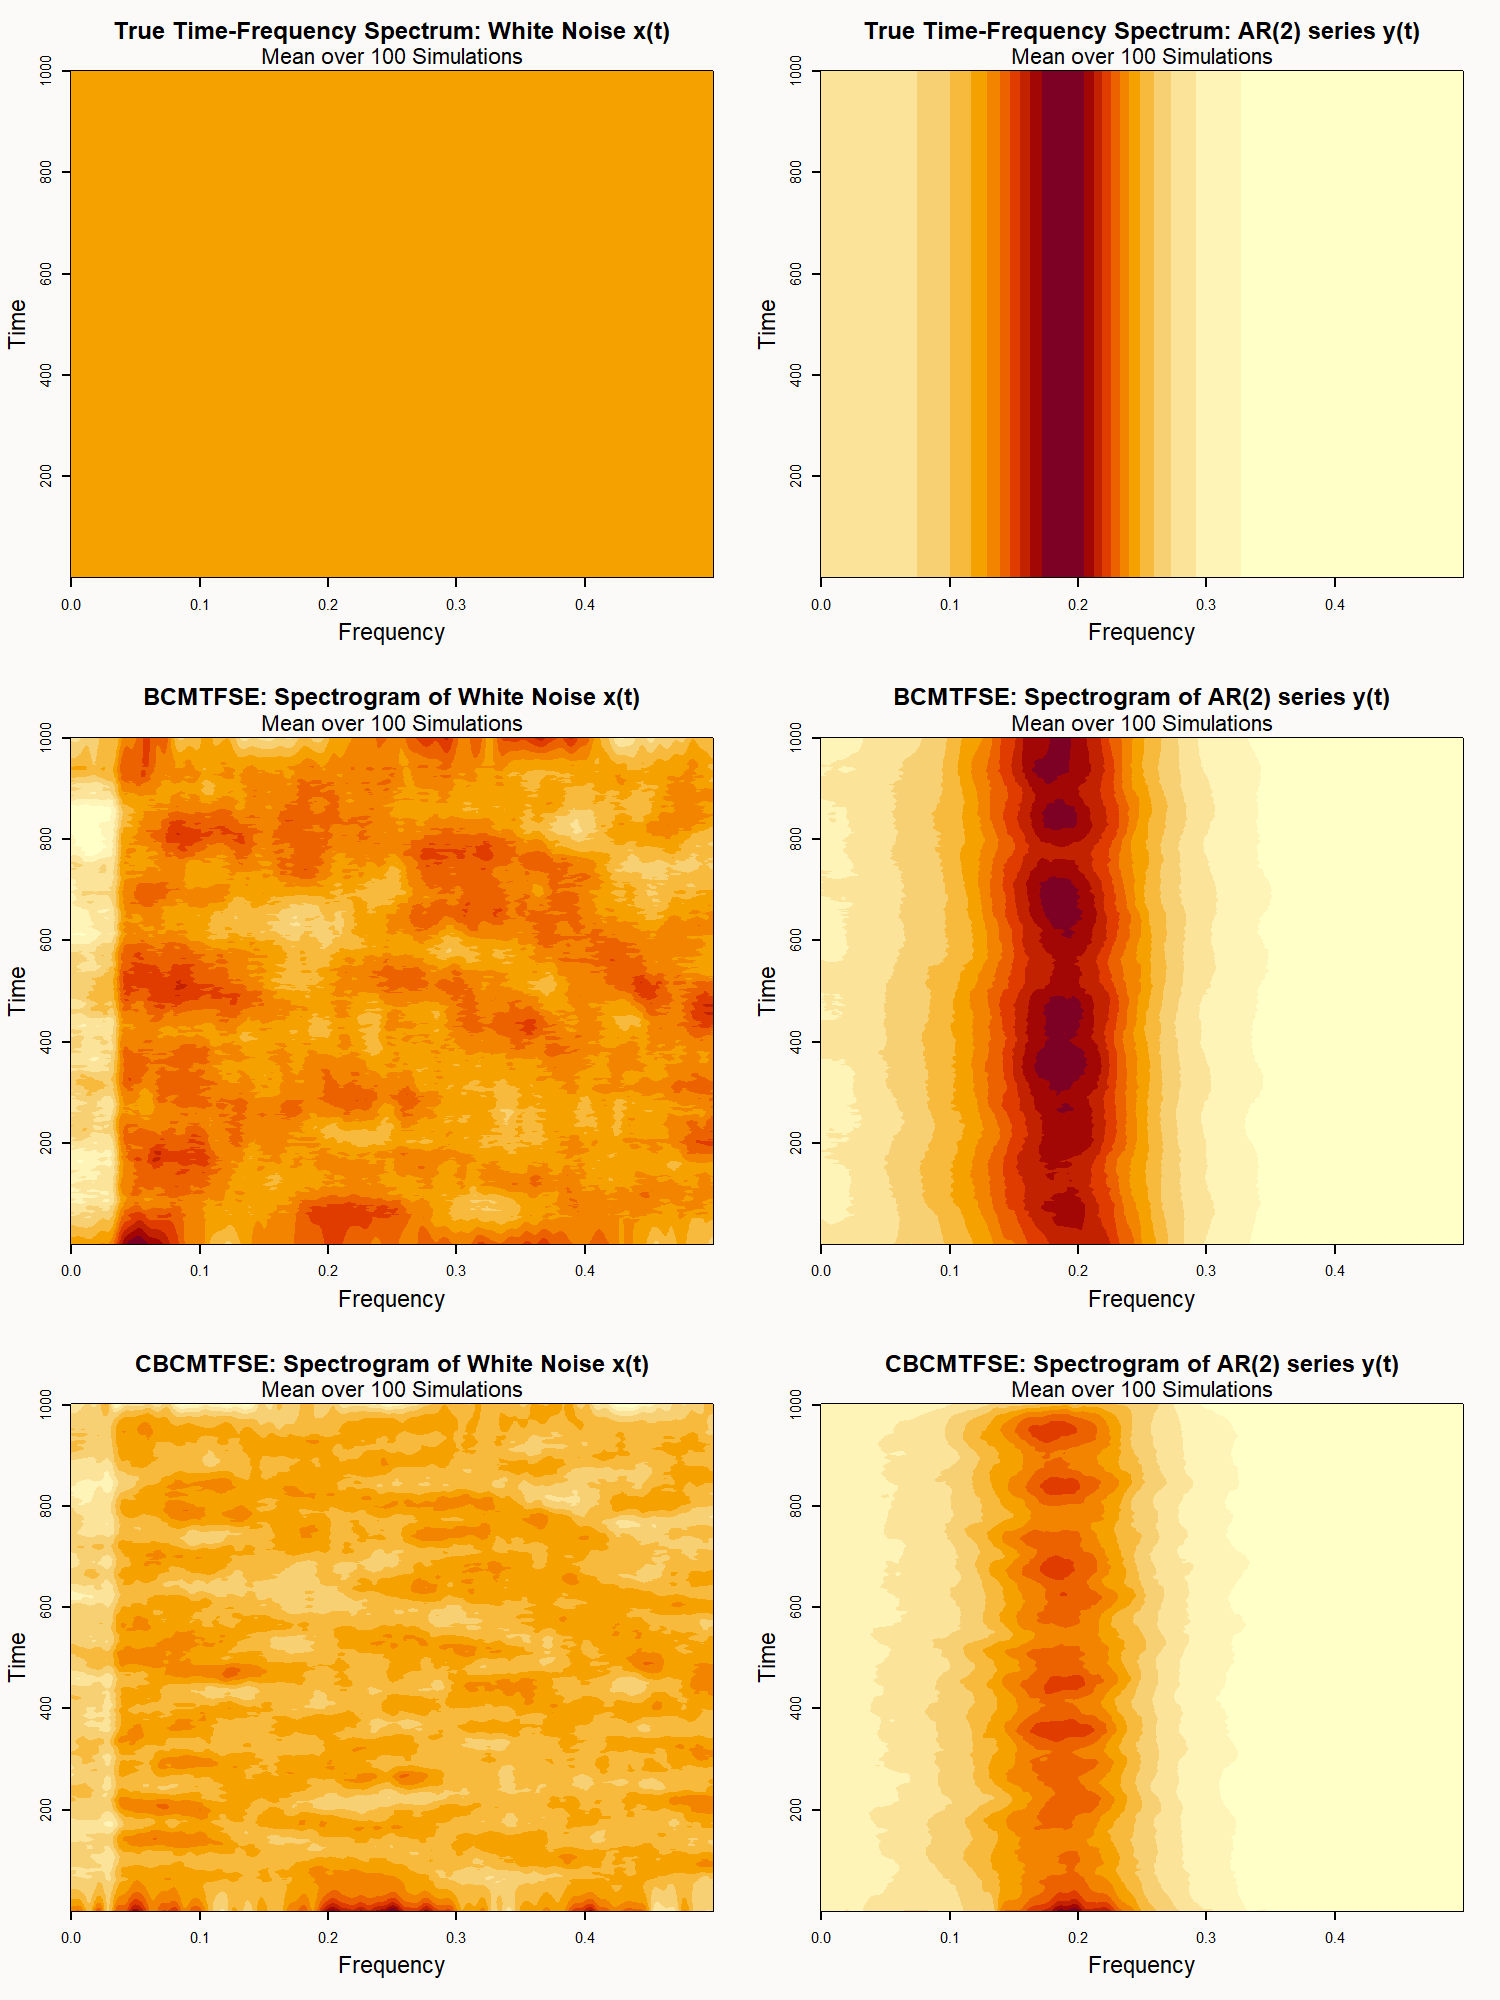
\includegraphics[width=\linewidth]{Fig/sgrams_0.png}
    \caption{Caption}
    \label{fig:1}
\end{figure}

\subsubsection{Example: Uniformly Modulated Process 1}
In the previous section, aside from white noise, we considered a stationary AR(2) series. Now, let us examine how these estimators perform when a similar series is uniformly modulated to no longer be stationary. The series we'll use is exactly the one featured in [??] - this allows for a graphical sanity check in terms of accurately reproducing the BCMTFSE and its results.

Suppose we have the following time series:
\begin{flalign}
    X(t)        &= \left( 2 - \exp\left\{\frac{-(t-500)^2}{2(200)^2}\right\} \right) Y(t) \\& \notag \\
    Y(t)        &= 0.8\,Y(t-1) - 0.4\,Y(t-2) + \epsilon(t)                 \\
    \epsilon(t) &= w\big(0,\;\sigma_\epsilon^2 = 10^4\big).
\end{flalign}


As the reader can see, $X(t)$ is an UMP, $Y$ is a stationary AR(2) process, and $\epsilon$ is purely white noise. What follows are the images we get when we run the new series through the code used to acheive the set of figures from the previous section.

\subsubsection{Example: Uniformly Modulated Process 2}

\subsubsection{Example: Non-Stationary, Non-Uniformly Modulated Process}







% --- ESTIMATING C ---------
\section{Estimation Modulating Functions of UMPs}
% Motivation and Review
Consider a UMP's time frequency spectrum, restricted to discrete sets of both time and frequency such that the TFS can be represented by a matrix. Any given row of this matrix represents the frequency spectrum of the UMP at a fixed, corresponding time point. As we move through time, the proportional structure of that frequency spectrum remains intact, with peaks and troughs expanding and contracting in unison. This restriction affords mathematical advantages in that the modulating function responsible for the UMP's non-stationarity is captured in the relative values of the TFS from row to row. Previous work [??] has been done to develop estimates for said modulating function, however, the established techniques are limited in that BLABLABLA. This section examines alternative approaches to estimating the UMP's modulating function.

\subsection{Derivation of Techniques}
Consider the UMP $X(t) = c(t)Y(t), t \in T =\{1,\dots,N\}$,  where $Y(t)$ is stationary. We begin at time $t=1$ rather than $t=0$ so that $t$ corresponds to the $t^{th}$ row of the UMP's TFS matrix $-$ the latter object denoted by $S_X(t,f)$ for Fourier frequencies $f \in \{f_1, \dots, f_{N_f}\}$. If we are to take the sum over each row of $S_X$, we're left with a vector $V_X(t)$ representing the total spectral power at each timepoint $t$. 
\begin{flalign}
    V_X(t) &\define \sum_{i=1}^{N_f} S_X(t,f_i)
\intertext{Recall that since $X(t)$ is uniformly modulated, its TFS matrix is such that} 
    S_X(t,f) &= c^2(t)\cdot S_Y(f),
\intertext{where $c^2$ is a column vector, and $S_Y$ is a row vector representing the spectrum of $Y$ (note $S_Y$ is time-independent thanks to $Y's$ stationarity). The structure of $V_X$ over time will resemble that of the squared modulating function to some extent. Namely, the proportion between any two entries in $V_X$ should reflect the proportions of the two entries of $c^2$ corresponding to those times.}\notag\\[-22pt] 
\intertext{\indent To estimate $c^2(t),$ then, an approach might be to examine each $V_X(t)$ as a proportion of $V_X(1)$, and simply store those proportions as a function of time. In fact, this can be done relative to any $t_0 \in T$,}
d_{t_0}(t) &\define V_X(t)/V_X(t_0).
\end{flalign}
The caveat, here, is that the above can only be constructed up to some normalizing constant. Namely, $d_{t_0}(t)$ at time $t = t_0$ is forced to have unit value. 

Although the issue of relying on a normalizing constant remains, a general improvement on the estimate $\hat c^2 = d_1$ (where $t_0=1$ is used without loss of generality) can be made by utilizing the information from every possible $d_t$. Notice that for $1 < k \leq N$,
\begin{flalign}
    c(1)^2 &= d_k(1)c(k)^2.
\intertext{If we sum both sides over k and divide by N-1,}
    c(1)^2 &= \frac{\sum_{k=2}^{N}d_k(1) \, c(k)^2}{(N-1)}    \\
           &\;\;\vdots \notag                                 \\
    c(N)^2 &= \frac{\sum_{k=2}^{N}d_k(N) \, c(k)^2}{(N-1)}    \\
\end{flalign}
N unknowns, N equations. Matrix for system of equations:

$$
A_{ij} = \frac{-rowsum\; i}{rowsum\;j} \qquad \text{(1's on diagonal)} \\
c = \Big[c(1)^2, \dots, c(N)^2\Big]' \\ \; \\
\text{solve: Ac = 0}
$$

\subsection{Performance using Simulated Data}

\end{document}